\documentclass[conference]{IEEEtran}
\usepackage[T1]{fontenc}
\usepackage[utf8]{inputenc}
\usepackage{lmodern,amsmath,booktabs,graphicx,xcolor,hyperref}
\renewcommand{\ttdefault}{lmtt}
\graphicspath{{figures/}}
\title{A Selectivity-Driven Adaptive Query Processing Engine for Hybrid SQL--Vector Databases}
\author{\IEEEauthorblockN{Anonymous Author}
\IEEEauthorblockA{\textit{Department of Computer Science and Engineering}\\
\textit{Vellore Institute of Technology, Chennai}\\
Chennai, India}}

\begin{document}
\maketitle

\begin{abstract}
Hybrid SQL--vector workloads admit multiple execution strategies whose latency and recall behavior vary with predicate selectivity. We present a PostgreSQL/pgvector prototype that combines PostgreSQL \texttt{EXPLAIN (FORMAT JSON)} selectivity estimates, empirical bucket-median latency calibration, conservative minimum-observed Recall@10 feasibility checks, and execution-plan verification to select among four candidate strategies. On the held-out workload, the conservative minimum-recall feasibility gate admitted only the exact SQL\_FIRST path: every approximate strategy exhibited at least one calibration observation below the 0.95 Recall@10 threshold in each populated selectivity bucket, so the policy selected SQL\_FIRST for all 250 held-out queries while measured approximate alternatives reached mean Recall@10 of only 0.76--0.81. The evaluation uses a 500-query synthetic relational workload over the SIFT1M dataset, with randomized predicates over category, price, and stock attributes and query vectors sampled from the SIFT1M vector collection. To prevent calibration leakage, the workload is partitioned into a disjoint 250-query calibration set and a disjoint 250-query held-out test set. Calibration statistics are constructed exclusively from the calibration set, while the held-out set is used to evaluate fixed strategies and the adaptive decision rule. This design provides a rigorous basis for reporting strategy-only latency and Recall@10 without asserting any numerical outcome before the benchmark results are analyzed.
\end{abstract}

\noindent\textit{Index Terms---}adaptive query processing, hybrid SQL--vector queries, PostgreSQL, pgvector, approximate nearest-neighbor search, selectivity estimation.

\section{Introduction}
Hybrid SQL--vector retrieval combines a relational predicate with nearest-neighbor ranking. A database can filter rows before exact ranking, retrieve ANN candidates before filtering, or invoke an ANN access path while applying the predicate. The latency of these alternatives can vary with predicate selectivity, while a fast approximate path can fail a required filtered-recall target. Exact filtering is recall-safe but may incur higher latency. Thus, a single fixed physical strategy is not necessarily appropriate for every hybrid query.

This paper studies a conservative safety layer for a PostgreSQL/pgvector prototype. The layer obtains a PostgreSQL \texttt{EXPLAIN (FORMAT JSON)} estimate, maps it to a fixed selectivity bucket, consults empirical latency and recall evidence for that bucket, rejects ANN strategies whose observed recall evidence does not satisfy the target, and records the expected ANN plan/index evidence. The central question is: \emph{on a held-out workload, can a selectivity-aware policy enforce the specified Recall@10 feasibility target while selecting among alternative hybrid execution paths?}

Our contributions are deliberately narrow and evidence-based. First, we describe a selectivity-driven strategy-selection layer that calibrates four PostgreSQL/pgvector candidates, with the evaluated adaptive policy selecting the exact SQL\_FIRST fallback for every held-out query, because no approximate strategy satisfied the minimum-observed-recall bar in any populated bucket. Second, we formalize a conservative decision rule that combines planner-estimated selectivity, empirical bucket-median latency calibration, and minimum-observed recall feasibility. Third, we include an execution-plan verification check for ANN access paths. Fourth, we evaluate the resulting latency--recall tradeoff using a disjoint calibration and held-out test design over a 500-query SIFT1M workload. We do not claim optimality, generalization, state-of-the-art performance, or production readiness; quantitative conclusions are reserved for the measured benchmark results.

\section{Related Work}
Relational optimizers depend on cardinality estimates and cost models when selecting plans; errors in these components remain a central query-optimization issue \cite{optimizer_survey}. PostgreSQL supplies the relational planning and \texttt{EXPLAIN} facilities used here \cite{postgresql16}. Learned optimizers such as Bao adapt optimizer steering from feedback \cite{bao}; our prototype is intentionally simpler: it uses frozen empirical summaries rather than a learned model or online updates.

For vector retrieval, HNSW is a graph-based ANN method \cite{malkov2020hnsw}, and IVFFlat is a pgvector-supported approximate index access method \cite{pgvector}. Filtered vector search has been characterized in terms of pre-, post-, and inline filtering, with selectivity and predicate--vector correlation affecting the tradeoff \cite{filtered_vector_search}. The present work evaluates PostgreSQL/pgvector execution choices rather than proposing a new ANN index or external-system comparison. SIFT1M provides the one-million-vector benchmark context \cite{faiss_sift1m}.

\section{Problem Definition}
Let a hybrid query be $q=\langle \mathbf{v},P,k\rangle$, where $\mathbf{v}$ is a query vector, $P$ is a relational predicate, and $k=10$. Let $\hat{\sigma}(P)$ denote PostgreSQL's pre-execution selectivity estimate. This differs from measured selectivity, which is available only after execution and is never a planner input. For each strategy $s\in\mathcal{S}$, calibration supplies $\widehat{L}_s(b)$, the median strategy-only latency in selectivity bucket $b$, and observed recall evidence $R^{\min}_s(b)$. The policy chooses
\begin{align}
s^*(q) &= \arg\min_{s\in\mathcal{F}(b)}\widehat{L}_s(b), \\
\mathcal{F}(b) &= \{\texttt{SQL\_FIRST}\}\cup
\{s:R^{\min}_s(b)\geq0.95\}.
\end{align}
where $b$ contains $\hat{\sigma}(P)$. The notation describes a decision based on calibration evidence; it does not imply knowledge of post-execution latency or recall. \texttt{SQL\_FIRST} is always feasible because it produces the exact filtered reference.

\section{System Architecture}
\subsection{Hybrid SQL--Vector Query Model}
Predicates are translated into parameterized SQL and combined with L2 vector ordering. The system keeps relational filtering and vector access within PostgreSQL/pgvector execution.

\subsection{Selectivity Estimation}
For each query, PostgreSQL \texttt{EXPLAIN (FORMAT JSON)} supplies the planning selectivity estimate \cite{postgresql16}. The planner never uses the measured post-execution selectivity as its input.

\subsection{Strategy Space}
The candidate strategies are \texttt{SQL\_FIRST}, \texttt{VECTOR\_FIRST\_HNSW}, \texttt{HNSW\_HYBRID}, and \texttt{IVFFLAT\_HYBRID}. \texttt{SQL\_FIRST} is the exact fallback.

\subsection{Latency Calibration}
For each strategy and selectivity bucket, the prototype uses the empirical median observed strategy-only latency as its calibration estimate. These bucket medians are descriptive summaries, not a causal performance model.

\subsection{Recall@10 Feasibility}
A non-exact strategy is eligible only when its observed minimum Recall@10 in the relevant calibration bucket meets 0.95. This is conservative observed evidence, not a guarantee for unobserved workloads.

\section{Adaptive Strategy Selection Method}
\subsection{Decision Rule and Execution}
For a query, the planner: (1) obtains $\hat{\sigma}(P)$ from \texttt{EXPLAIN}; (2) maps it to a fixed bucket; (3) retrieves each strategy's median latency and recall evidence; (4) excludes non-exact strategies whose observed bucket minimum Recall@10 is below 0.95, or has insufficient evidence; (5) selects the lowest calibrated latency among the remaining strategies; (6) retains \texttt{SQL\_FIRST} as a deterministic exact fallback; (7) executes; and (8) records strategy-only latency and Recall@10 against the exact reference. ANN executions additionally require the intended index in separately recorded plan evidence.

\begin{figure*}[t]
\centering\includegraphics[width=.83\textwidth]{figure_01_decision_flow.pdf}
\caption{Adaptive execution decision flow. PostgreSQL EXPLAIN supplies an estimated selectivity; empirical latency calibration and conservative recall-feasibility evidence guide selection from a four-strategy candidate set; on the evaluated workload, only SQL\_FIRST was selected. \texttt{SQL\_FIRST} is the exact fallback. The diagram describes the process and does not imply globally optimal selection.}
\label{fig:architecture}
\end{figure*}

\section{Implementation}
\subsection{PostgreSQL/pgvector}
The evaluated implementation used PostgreSQL~16.14 and pgvector~0.8.5. All quantitative results in this paper are from the PostgreSQL/pgvector artifacts, not legacy hnswlib/pandas outputs.

\subsection{SIFT1M Dataset}
The dataset contains 1,000,000 vectors of dimension 128. Distance is L2.

\subsection{SQL\_FIRST}
\texttt{SQL\_FIRST} applies the relational predicate and performs exact vector ordering; it is the recall-safe fallback.

\subsection{VECTOR\_FIRST\_HNSW}
\texttt{VECTOR\_FIRST\_HNSW} retrieves HNSW vector candidates and applies the predicate after candidate retrieval. The evaluated candidate budget was 100.

\subsection{HNSW\_HYBRID}
\texttt{HNSW\_HYBRID} executes the hybrid query using the HNSW access path with the experiment's frozen pgvector settings. The artifacts do not support treating a particular setting as a generally tuned configuration.

\subsection{IVFFLAT\_HYBRID}
\texttt{IVFFLAT\_HYBRID} executes the hybrid query using the IVFFlat access path with the experiment's configured pgvector settings.

\subsection{Plan Verification}
ANN strategy records require their intended index in the recorded plan evidence for admission-time verification. When the planner instead serves a query through an exact bitmap or sequential path --- which it may legitimately do on highly selective predicates --- this is recorded via an access-path field rather than counted as a verification failure. Verification demonstrates compliance with the experiment's access-path rule, not performance correctness or generalization.

\section{Experimental Methodology}
\subsection{Dataset and Workload}
The evaluation uses the SIFT1M dataset containing 1,000,000 vectors of dimension 128 with L2 distance. It generates 500 hybrid queries, each pairing a query vector sampled from the SIFT1M vector collection with a randomized relational predicate over the synthetic attributes \texttt{category}, \texttt{price}, and \texttt{in\_stock}. Predicate parameters are randomized over targets spanning $[0.01,1.0]$. Because predicate shape is tied to the target interval and PostgreSQL's estimates are driven by three attribute statistics, realized planning-time estimates concentrate in three bands ($\leq$0.05, 0.10--0.25, $>$0.50); two selectivity buckets receive no queries on this workload (Section~\ref{sec:limitations}). All queries request $k=10$ nearest neighbors, and Recall@10 is computed against an exact filtered \texttt{SQL\_FIRST} reference.

\subsection{Hardware and Software}
The frozen artifact records PostgreSQL~16.14 and pgvector~0.8.5. The provenance manifest contains available host/package metadata, but it was collected after the run and is not a complete hardware characterization.

\subsection{Metrics}
Strategy-only latency times selected SQL execution and is the comparable latency metric. Recall@10 is the overlap with the exact filtered top-10 reference. We report mean, median, P95, minimum recall, and fraction meeting Recall@10 $\geq0.95$.

\subsection{Calibration}
The 500-query workload is partitioned before execution into two disjoint sets: 250 calibration queries and 250 held-out test queries. The calibration phase executes all four candidate strategies, \texttt{SQL\_FIRST}, \texttt{VECTOR\_FIRST\_HNSW}, \texttt{HNSW\_HYBRID}, and \texttt{IVFFLAT\_HYBRID}, and constructs an in-memory map keyed by strategy and estimated-selectivity bucket. Each entry stores the calibration median strategy-only latency and minimum observed Recall@10. No held-out query, latency, recall, or plan observation is used to construct this map.

\subsection{Experimental Protocol}
For each held-out query, the harness first invokes PostgreSQL \texttt{EXPLAIN (FORMAT JSON)} to obtain the planning-time selectivity estimate and map the query to a calibration bucket. It then executes each of the four fixed strategies exactly five times. Strategy-only latency excludes EXPLAIN and planning overhead; the reported per-query latency is the median across the five repetitions. Recall@10 is computed by comparing each result's top-10 IDs with the exact \texttt{SQL\_FIRST} result for the same query. The adaptive policy is selected using only the held-out query's EXPLAIN estimate and the frozen calibration map, and is evaluated against the fixed-strategy measurements.

\subsection{Reproducibility Checklist}
The frozen artifacts identify SIFT1M (1,000,000 vectors, 128 dimensions, L2), PostgreSQL~16.14, pgvector~0.8.5, the 500-query workload, the 250/250 split, $k=10$, the four strategies, fixed selectivity buckets, the recall target, and the exact filtered reference. They preserve predicate-generation parameters, random seeds, \texttt{EXPLAIN} estimates, calibration summaries, per-query held-out outputs, and plan evidence. These artifacts support independent reconstruction of the calibration/test boundary and evaluation protocol.

\section{Results}
\subsection{Fixed Strategy Comparison}
Table~\ref{tab:strategy-comparison} shows the observed tradeoff. \texttt{HNSW\_HYBRID} has the lowest mean strategy-only latency (2.3~ms) but its mean Recall@10 is only 0.810, with individual observations as low as 0.0; 30.0\% of its observations fall below the 0.95 target. The adaptive policy reports Recall@10 of 1.000 on all 250 held-out queries; because the minimum-recall gate excluded every approximate strategy in every populated bucket, its latency is identical to \texttt{SQL\_FIRST}'s (mean 99.0~ms, median 94.7~ms, P95 179.0~ms).
\begin{table*}[t]
\centering
\caption{Observed strategy-only performance on the 250-query held-out test workload. Recall@10 is the mean over 250 queries; Min recall and Frac $\geq$0.95 are computed over the same observations.}
\label{tab:strategy-comparison}
\scriptsize
\begin{tabular}{lrrrrrr}
\toprule
Strategy & Mean ms & Median ms & P95 ms & Recall@10 & Min recall & Frac $\geq$0.95 \\
\midrule
Adaptive & 99.0 & 94.7 & 179.0 & 1.000 & 1.000 & 1.000 \\
SQL\_FIRST & 99.0 & 94.7 & 179.0 & 1.000 & 1.000 & 1.000 \\
VECTOR\_FIRST\_HNSW & 3.5 & 2.4 & 9.2 & 0.763 & 0.000 & 0.656 \\
HNSW\_HYBRID & 2.3 & 1.4 & 3.8 & 0.810 & 0.000 & 0.700 \\
IVFFLAT\_HYBRID & 5.7 & 4.7 & 13.9 & 0.813 & 0.100 & 0.352 \\
\bottomrule
\end{tabular}
\end{table*}


\subsection{Latency and Selectivity}
Figure~\ref{fig:latency-selectivity} plots raw observed points against PostgreSQL-estimated selectivity. It demonstrates heterogeneous observed behavior, not a fitted latency/selectivity law.
\begin{figure}[t]
\centering
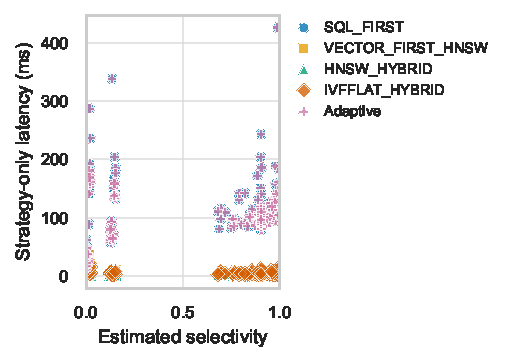
\includegraphics[width=\columnwidth]{figure_1_latency_vs_selectivity.pdf}
\caption{Observed strategy-only latency by PostgreSQL-estimated selectivity on the 250-query held-out test set. Raw points show heterogeneous strategy behavior; no mathematical latency/selectivity relationship is claimed.}
\label{fig:latency-selectivity}
\end{figure}

\subsection{Recall@10 and Selectivity}
Figure~\ref{fig:recall-selectivity} summarizes the 250 adaptive observations, including its \texttt{SQL\_FIRST} selections. The reported adaptive Recall@10 was 1.000. Across the 250 observations per fixed strategy, the fraction below the 0.95 target was 30.0\% for \texttt{HNSW\_HYBRID}, 64.8\% for \texttt{IVFFLAT\_HYBRID}, and 34.4\% for \texttt{VECTOR\_FIRST\_HNSW}. This is descriptive evaluated-workload evidence, not proof of generalization.
\begin{figure}[t]
\centering
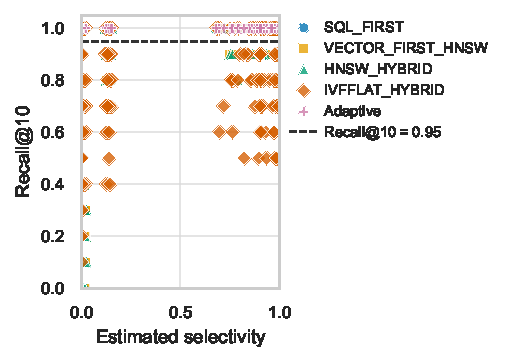
\includegraphics[width=\columnwidth]{figure_2_recall_vs_selectivity.pdf}
\caption{Recall@10 by PostgreSQL-estimated selectivity on the 250-query held-out test set. Adaptive observations are shown; the dashed line is the 0.95 target. Several fixed ANN observations are below target on the evaluated workload.}
\label{fig:recall-selectivity}
\end{figure}

\subsection{Adaptive Strategy Selection}
The gate selected \texttt{SQL\_FIRST} for all 250 held-out queries --- 60 in $[0.00,0.05)$, 37 in $[0.10,0.25)$, and 153 in $[0.50,1.00)$ --- and selected no approximate strategy in any bucket; two buckets received zero queries (Section~\ref{sec:limitations}). Table~\ref{tab:selection-by-bucket} and Figure~\ref{fig:bucket-selection} report descriptive counts rather than statistically significant bucket effects.
\begin{table}[t]
\centering
\caption{Adaptive selections across estimated-selectivity buckets on the 250-query held-out test set. The feasibility gate admitted only \texttt{SQL\_FIRST}; two buckets received no queries (see Section~\ref{sec:limitations}).}
\label{tab:selection-by-bucket}
\scriptsize
\resizebox{\columnwidth}{!}{%
\begin{tabular}{lrrrrr}
\toprule
Bucket & Queries & SQL\_FIRST & VECTOR\_FIRST\_HNSW & HNSW\_HYBRID & IVFFLAT\_HYBRID \\
\midrule
$\leq5\%$ & 60 & 60 & 0 & 0 & 0 \\
$5$--$10\%$ & 0 & 0 & 0 & 0 & 0 \\
$10$--$25\%$ & 37 & 37 & 0 & 0 & 0 \\
$25$--$50\%$ & 0 & 0 & 0 & 0 & 0 \\
$>50\%$ & 153 & 153 & 0 & 0 & 0 \\
\midrule
Total & 250 & 250 & 0 & 0 & 0 \\
\bottomrule
\end{tabular}}
\end{table}

\begin{figure}[t]
\centering
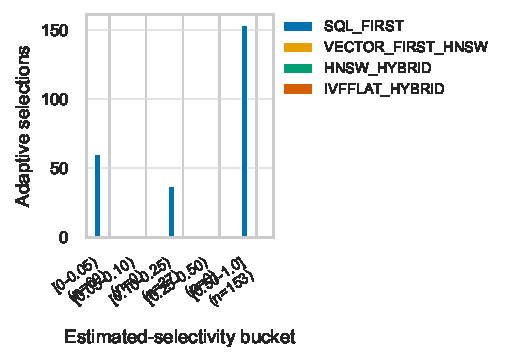
\includegraphics[width=\columnwidth]{figure_3_adaptive_selections_by_bucket.pdf}
\caption{Adaptive strategy selections across estimated-selectivity buckets. Labels give evaluated-workload sample counts and do not support population or significance claims.}
\label{fig:bucket-selection}
\end{figure}

\subsection{Decision Overhead}
The adaptive decision-to-verified-execution wall time had mean 134.36~ms, median 100.41~ms, and P95 317.54~ms. It includes EXPLAIN, planning, and verified execution wall time, so it is not directly comparable to strategy-only latency. Component decomposition attributes 133.08~ms of the mean overhead to the selected strategy's execution itself, while EXPLAIN and the bucket-lookup/calibration decision contribute only ${\sim}1.3$~ms combined. This overhead records a single per-query wall-clock execution (the first repetition), whereas Table~\ref{tab:strategy-comparison} reports the median across five repetitions; because the gate selected \texttt{SQL\_FIRST} for every query, this single cold-path execution exceeds the median-of-repetitions figure (99.0~ms), a cache-state effect consistent with the timing sensitivity noted in Section~\ref{sec:limitations}.
\begin{table}[t]
\centering
\caption{Adaptive decision-to-verified-execution wall time per held-out query (EXPLAIN + calibration decision + verified execution of the selected strategy, single execution per query). Not directly comparable to the median-of-repetitions strategy-only latency in Table~\ref{tab:strategy-comparison}.}
\label{tab:decision-overhead}
\small
\begin{tabular}{rrr}
\toprule
Mean ms & Median ms & P95 ms \\
\midrule
134.36 & 100.41 & 317.54 \\
\bottomrule
\end{tabular}
\end{table}


\subsection{Plan Verification}
Of 750 recorded fixed ANN executions, 728 used their named ANN access path; the remaining 22 were planner-chosen exact bitmap scans on highly selective predicates, logged transparently via an access-path field rather than treated as failures. All 250 SQL\_FIRST executions avoided ANN indexes as required. Table~\ref{tab:plan-verification} documents this execution-integrity check.
\begin{table}[t]
\centering
\caption{Named-access-path verification for the 250-query held-out test set. ANN strategies are verified against their own index type; planner-chosen exact bitmap fallbacks are logged separately via the access-path field rather than counted as failures.}
\label{tab:plan-verification}
\scriptsize
\resizebox{\columnwidth}{!}{%
\begin{tabular}{lrr}
\toprule
Execution scope & Records & Named path verified \\
\midrule
Adaptive ANN selections & 0 & 0 \\
Fixed SQL\_FIRST & 250 & 250 \\
Fixed VECTOR\_FIRST\_HNSW & 250 & 250 \\
Fixed HNSW\_HYBRID & 250 & 238 \\
Fixed IVFFLAT\_HYBRID & 250 & 240 \\
All ANN executions & 750 & 728 \\
SQL\_FIRST executions (no ANN required) & 250 & 250 \\
\bottomrule
\end{tabular}}
\end{table}


\section{Discussion}
The results section reports fixed-strategy and adaptive-policy measurements on the held-out test workload. The comparison is interpreted through the safety layer: approximate strategies are admitted only when calibration evidence in the corresponding selectivity bucket satisfies the recall feasibility threshold, while exact SQL-first remains available as a fallback. Latency and recall observations are therefore evaluated separately from the calibration phase.

\section{Threats to Validity and Limitations}\label{sec:limitations}
The disjoint calibration and held-out test sets remove workload-level calibration leakage, but timing remains sensitive to cache state, execution order, hardware, and ANN parameters. The synthetic predicates and SIFT1M vectors limit direct generalization to other data distributions and application workloads. Feasibility remains an empirical summary of calibration evidence rather than a guarantee for arbitrary workloads, and the held-out results should be interpreted within the tested PostgreSQL/pgvector configuration. Three further limitations are specific to this evaluation. First, two of the five selectivity buckets ([0.05,0.10) and [0.25,0.50)) received zero calibration and zero held-out queries, because PostgreSQL's estimates for the three fixed predicate templates never fall in those ranges; all results therefore cover only the three populated buckets. Second, the minimum-based admission rule is sensitive to individual tail observations at these sample sizes: in [0.10,0.25), HNSW\_HYBRID's rejection traces to a single 0.40 observation among 38 otherwise-perfect calibration runs, whereas in [0.00,0.05) the majority of observations (46 of 56) are genuinely below 0.5. Third, because the gate admitted no approximate path, this evaluation provides no end-to-end evidence about adaptive ANN execution quality; it establishes only that the safety layer refused every approximate admission on observed evidence.

\section{Future Work}
The more ambitious SDAO design described in the companion protocol document motivates several extensions, but those designs were not implemented in the current PostgreSQL/pgvector prototype and are not part of the evidence reported here. A stronger evaluation should use disjoint tuning, calibration, and held-out test workloads; repeated randomized or paired trials; separate warm- and cold-cache reporting; confidence intervals; more queries and datasets; and hardware sensitivity analyses. Additional work can measure HNSW \texttt{ef\_search}, IVFFlat probe, and vector-first candidate-budget sensitivity; planner and memory overhead; and comparisons with external filtered-ANN systems. Learned selectivity or predicate--vector-overlap estimates, online calibration, and learned thresholds remain future directions rather than components of the current paper.

\section{Conclusion}
This exploratory PostgreSQL/pgvector prototype combines EXPLAIN-derived selectivity estimates, empirical bucket calibration, a conservative minimum-recall feasibility gate, and plan verification into a single safety layer for hybrid SQL--vector queries. On the evaluated workload the gate admitted only the exact \texttt{SQL\_FIRST} path for every held-out query: measured strategy-only latencies were 99.0~ms for \texttt{SQL\_FIRST} versus 3.5~ms for \texttt{VECTOR\_FIRST\_HNSW} ($\approx$28$\times$), 2.3~ms for \texttt{HNSW\_HYBRID} ($\approx$43$\times$), and 5.7~ms for \texttt{IVFFLAT\_HYBRID} ($\approx$17$\times$) --- an approximate-path latency advantage of roughly 17--43$\times$ depending on strategy, which the safety layer traded entirely for a guaranteed Recall@10 of 1.000 on this workload. The disjoint calibration and held-out evaluation design enabled this assessment without calibration leakage, but two of five selectivity buckets received no queries under the current predicate generator, and the min-based admission rule is sensitive to individual tail observations at these sample sizes. Quantifying when such conservatism is unnecessarily strict --- and whether relaxed admission rules can admit approximate paths safely at scale --- remains future work.

\appendix
\section{Supporting Figures}
\begin{figure*}[t]\centering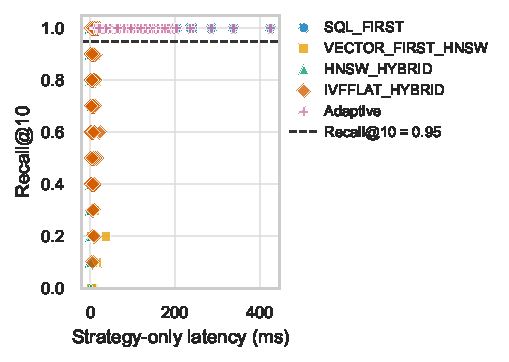
\includegraphics[width=.7\textwidth]{figure_4_latency_recall_tradeoff.pdf}
\caption{Observed strategy-only latency and Recall@10; the dashed line marks the required 0.95 target. This supporting exploratory plot is not evidence of statistical superiority.}\label{fig:tradeoff}\end{figure*}

\bibliographystyle{plain}
\bibliography{references}
\end{document}
